\documentclass{article}

% Math formulas
\usepackage{amsmath}

\usepackage{minted}


% Zeichenkodierung und Schriftart
\usepackage[utf8]{inputenc}
\usepackage[T1]{fontenc}
\usepackage{lmodern}

% TikZ
\usepackage{tikz}
\tikzset{
  level/.style={
    sibling distance=30mm/#1
  },
  level distance=10mm,
}

 \tikzset{
  every node/.style={
    draw,
    circle,
    inner sep=0pt,
    minimum width=15pt
  },
  thick
}


\begin{document}
\title{Dynamic Programming}
\author{Juan Andrés Osorio Escobar}
\date{\today}
\maketitle

\input{chapters/abstract.tex}
\tableofcontents

 
 \section{introduction}


What is dynamic programming? it really sounds like one of those big buzzwords that seem to
attract big audiences that tend to follow trends. But put in simple words, Dynamic Programming is just a tabular method, 
which reduces a lot of duplicate computations on a problem. Now, how does dynamic programming work? lets dive in with a simple example at first, the fibonacci numbers,
which form a sequence defined as follows:
  \\
  \[
    fib(n) = \left\{\begin{array}{lr}
      n, & \text{for } n = 1, n = 2\\
      fib(n-1) + fib(n-2), & \text{otherwise}
      \end{array}\right\}
  \]
  \\

we could write a simple program to compute the nth fibonacci number as follows:

\begin{minted}{python}

def fibonacci(n):
  if (n <= 1):
    return n
  else :
    return fibonacci(n - 1) + fibonacci(n + 2)

\end{minted}


to get a rough picture of the space and time complexity for this program, we could depict the steps
the program would take to compute an arbitrary number n, in the form of a tree. For n = 6, we have:


\begin{figure}[ht]
  \centering
  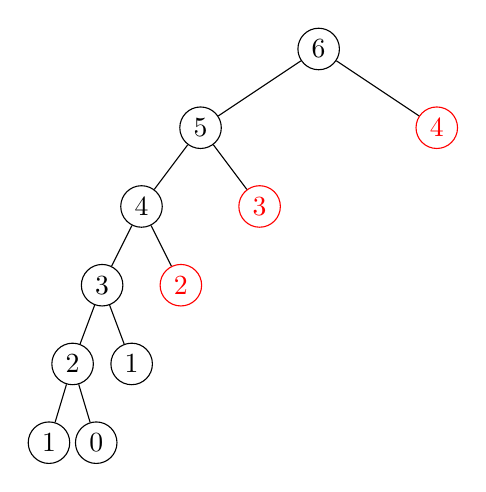
\begin{tikzpicture}
    \node {6}
      child { node {5}
        child { node {4} 
          child{ node {3} 
            child { node {2}
              child {node {1}}
              child {node {0}}
            }
            child { node {1}}
          }
          child{ node[color=red] {2} }
        }
        child { node[color=red] {3} }
      }
      child { node[color=red] {4}
      };
  \end{tikzpicture}
  \caption{Fibonacci recursion tree with $n = 6$}
  \label{fig:fib1}
\end{figure}

The red nodes in figure \ref{fig:fib1} still have to be visited by the algorithm, and they are expanded all 
way down into a node with label one or zero, even though if the answer was already computed in any other 
branch of the tree. This repetitive computation slows down the program drastically as n grows,
you can see that the number of nodes grows exponentially, since for every level we traverse down,
the number of nodes potentially double: the time complexity for this algorithm is $O(2^n)$, which is 
the number of nodes.

\begin{figure}[ht]
  \centering
  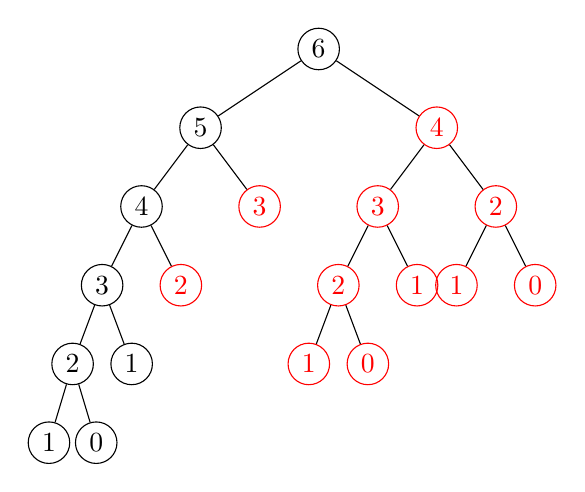
\begin{tikzpicture}
    \node {6}
      child { node {5}
        child { node {4} 
          child{ node {3} 
            child { node {2}
              child {node {1}}
              child {node {0}}
            }
            child { node {1}}
          }
          child{ node[color=red] {2}}
        }
        child { node[color=red] {3}}
      }
      child { node[color=red] {4}
        child{ node[color=red] {3} 
            child { node[color=red] {2}
              child {node[color=red] {1}}
              child {node[color=red] {0}}
            }
            child { node[color=red] {1}}
          }
        child{ node[color=red] {2} 
            child {node[color=red] {1}}
            child {node[color=red] {0}}
        }
      };
  \end{tikzpicture}
  \caption{Expanded fibonacci recursion tree}
  \label{fig:fib2}
\end{figure}

in figure \ref{fig:fib2} we expanded one of the red nodes labeled with 4: it gets computed twice, completely.
expanding all the tree would show us that node 3 gets computed three times, node 2 gets computed five times.
if we chose n = 7, for example, node 2 would be computed eight times. This unnecessary repeated
computations are  what makes this algorithm so slow.

Now, what if instead of repeating all this computations, the answers are stored somewhere? Each
time the algorithm would start , it wouldinstead look up in some kind of record or table, 
and if it finds a value, it just simply returns the value found immediatly.


\begin{minted}{python}
# initialize the look up table with 
# non-recursively defined fibonacci numbers.
look_up_table = {
 0: 1,
 1: 1  
}

def dp_fibonacci(n):
  if (look_up_table.at(n)):
    return look_up_table.at(n)
  else :
    look_up_table[n] = dp_fibonacci(n - 1) + dp_fibonacci(n + 2)
    return look_up_table[n]
\end{minted}


applying this change to the algorithm, yields a linear run time $O(n)$. This is because instead of expanding the
nodes marked red, dp\_fibonacci just retrieves the value from a dictionary, which is $O(1)$. This
is a tremendous gain in performance.




\end{document}